% !TeX program = xelatex
% ============================================================================
%  实 Grassmann 流形的欧氏非嵌入问题
%  —— 由 Notion 主稿（page id 411ecac8-3544-81e4-8480-ceb337f02db0）复写
%  编译：xelatex main.tex （两遍，生成目录与交叉引用）
%  说明：本工程只做语法与排版层面的重整，不改变原文的数学内容与结论。
% ============================================================================
\documentclass[11pt,a4paper,UTF8]{ctexart}

% ---------- 页面与版式 ----------
\usepackage[a4paper,left=2.6cm,right=2.6cm,top=2.8cm,bottom=2.8cm]{geometry}
\usepackage{fancyhdr}
\usepackage{emptypage}
\linespread{1.28}
\setlength{\parskip}{0.28em}

% ---------- 数学 ----------
\usepackage{amsmath,amssymb,amsthm,mathtools,bm}
\usepackage{mathrsfs}
\allowdisplaybreaks[2]
\numberwithin{equation}{section}

% ---------- 表格与图形 ----------
\usepackage{booktabs,array,multirow,makecell,tabularx}
\usepackage{placeins}   % \FloatBarrier：防止表格漂到下一节标题之后
\usepackage{tikz}
\usetikzlibrary{arrows.meta}
\usepackage{capt-of}   % 非浮动图形的 \captionof
\usepackage{enumitem}
\setlist{itemsep=0.15em,topsep=0.35em,parsep=0pt}

% ---------- 强调框 ----------
\usepackage[most]{tcolorbox}
\newtcolorbox{scope}{enhanced,breakable,colback=black!3,colframe=black!55,
  boxrule=0.6pt,arc=2pt,left=8pt,right=8pt,top=6pt,bottom=6pt,
  fonttitle=\bfseries,title=文档定位}

% ---------- 颜色与超链接 ----------
\usepackage{xcolor}
\definecolor{linknavy}{RGB}{22,64,124}
\definecolor{citegreen}{RGB}{27,102,74}
\definecolor{urlgray}{RGB}{92,62,120}
\usepackage[colorlinks=true,
  linkcolor=linknavy, citecolor=citegreen, urlcolor=urlgray,
  bookmarksnumbered=true, bookmarksopen=true,
  pdftitle={实 Grassmann 流形的欧氏非嵌入问题},
  pdfauthor={瞿楚杰},
  pdfsubject={《文献阅读与课题调研》课程读书报告},
  pdfkeywords={实 Grassmann 流形, Stiefel--Whitney 类, 欧氏嵌入, 浸入, Schubert 类, Gr\"obner 基}
]{hyperref}

% ---------- 目录紧凑化（避免目录溢到第二页） ----------
\usepackage{tocloft}
\setlength{\cftbeforesecskip}{3pt}
\setlength{\cftbeforesubsecskip}{0.5pt}

% ---------- 定理环境（中文） ----------
\theoremstyle{plain}
\newtheorem{theorem}{定理}[section]
\newtheorem{proposition}[theorem]{命题}
\newtheorem{lemma}[theorem]{引理}
\newtheorem{corollary}[theorem]{推论}
\theoremstyle{definition}
\newtheorem{definition}[theorem]{定义}
\newtheorem{example}{例}[section]
\theoremstyle{remark}
\newtheorem{remark}{注}[section]
\newtheorem*{remark*}{注}

\renewcommand{\proofname}{证明}
\renewcommand\qedsymbol{$\square$}
% 允许“证明（……）”标题
\makeatletter
\renewenvironment{proof}[1][\proofname]{\par
  \pushQED{\qed}%
  \normalfont \topsep6\p@\@plus6\p@\relax
  \trivlist
  \item[\hskip\labelsep\itshape #1\@addpunct{.}]\ignorespaces
}{%
  \popQED\endtrivlist\@endpefalse
}
\makeatother

% ---------- 常用记号 ----------
\newcommand{\R}{\mathbb{R}}
\newcommand{\F}{\mathbb{F}}
\newcommand{\Ftwo}{\mathbb{F}_2}
\newcommand{\eps}{\varepsilon}
\newcommand{\GK}{G_{k,n}}
\newcommand{\cG}{\gamma}
\newcommand{\cGc}{\gamma^{\perp}}
\newcommand{\emb}{\hookrightarrow}
\newcommand{\nemb}{\not\hookrightarrow}
\newcommand{\imm}{\looparrowright}
\newcommand{\wbar}{\bar w}
\newcommand{\sw}[1]{w_{#1}}
\newcommand{\Schubert}[1]{\left(#1\right)}
\DeclareMathOperator{\Flag}{Flag}
\DeclareMathOperator{\Hom}{Hom}
\DeclareMathOperator{\embdim}{embdim}
\DeclareMathOperator{\imdim}{i}
\newcommand{\tb}[1]{\textbf{#1}}

% ---------- 页眉页脚 ----------
\pagestyle{fancy}
\fancyhf{}
\fancyhead[L]{\small\itshape 实 Grassmann 流形的欧氏非嵌入问题}
\fancyhead[R]{\small\thepage}
\renewcommand{\headrulewidth}{0.4pt}

% ============================================================================
\begin{document}

\begin{titlepage}
  \centering
  \vspace*{2.2cm}
  {\LARGE\bfseries 实 Grassmann 流形的欧氏非嵌入问题\par}
  \vspace{0.7cm}
  {\large\bfseries ——Stiefel--Whitney 类方法的系统整理与经典结果复现\par}
  \vspace{2.2cm}
  {\large 瞿楚杰\par}
  \vspace{0.5cm}
  {\normalsize《文献阅读与课题调研》课程读书报告\par}
  \vfill
  {\normalsize \today\par}
\end{titlepage}

\pagenumbering{roman}
% ============================================================================
%  摘要与关键词
% ============================================================================
\section*{摘要}
\addcontentsline{toc}{section}{摘要}
\markboth{摘要}{摘要}

本文围绕实 Grassmann 流形的欧氏非嵌入问题，系统整理典范丛、正交补丛、切丛公式与
Stiefel--Whitney 特征类之间的关系。对 $\GK=G_k(\R^{k+n})$，首先通过局部图像坐标
复现切丛同构 $T\GK\cong\Hom(\cG_k,\cGc_k)$；再由法丛的稳定平凡化说明：若闭流形
$M^d$ 嵌入 $\R^{d+c}$，则法丛的总 Stiefel--Whitney 类等于切丛总类的逆。由此，
非零的共轭类 $\wbar_j(TM)$ 为余维提供必要的下界；在闭流形的欧氏嵌入临界次数判据
下，它还排除余维恰等于 $j$ 的端点。本文特别强调：形式多项式的计算
必须在真实的 $H^*(\GK;\Ftwo)$ 商环中约化，且正交补丛的 Stiefel--Whitney 类、
切丛的共轭类、以及嵌入与浸入这三组概念不可混用。

在此基础上，本文核验并复现 Oproiu 关于 $G_{2,n}$ 与 $G_{3,n}$ 的代表性非嵌入
论证，说明二进制参数分段如何与 Schubert 类的非零性、以及欧氏嵌入的临界次数条件
相结合；同时整理 Hiller--Stong 关于实 Grassmann 流形浸入维数的命题与界，并将其
严格保持在 immersion 的语境之内。最后，通过 $G_{2,2}$ 等小参数例子展示
“总类公式——商环约化——非零性判定——环境维数排除”这一计算链条，并区分已知定理、
个人复现与尚待证明的探索性观察。本文的结论是：Stiefel--Whitney 类能够提供可靠的
非嵌入必要条件与浸入维数下界，但通常不足以单独决定最小的欧氏嵌入维数。

\vspace{0.8em}
\noindent\tb{关键词：}实 Grassmann 流形；典范丛；切丛；Stiefel--Whitney 类；
共轭特征类；Schubert 类；Gr\"obner 基；欧氏嵌入；浸入；法丛

\vspace{1.2em}
\begin{scope}
本文是《文献阅读与课题调研》课程的持续写作主稿，其目标是形成一份结构完整、
数学论证严谨、引用可核验、可提交的个人读书报告。每周的文献阅读属于研究准备，
其成果须写入本文，而不应只留下独立的阅读笔记。

写作遵循两条原则：其一，先形成可读的初稿，再随文献核验持续修订；其二，明确区分
已核验内容、待核验内容与个人探索。全文采用统一记号 $\GK=G_k(\R^{k+n})$，其维数
为 $kn$；若所引文献采用不同记号，引用时均明确给出转换关系。
\end{scope}

\clearpage

\tableofcontents
\clearpage
\pagenumbering{arabic}

% ============================================================================
%  记号与约定（全局记号表；不改动任何数学内容，只汇总正文已定义的符号）
% ============================================================================
\section*{记号与约定}
\addcontentsline{toc}{section}{记号与约定}
\markboth{记号与约定}{记号与约定}

本文自始至终使用下列记号。表中每一项在正文对应小节均有定义，此处仅作查阅之用；
若某项在个别文献中含义不同，引用时另行注明。

\begin{center}
\small
\renewcommand{\arraystretch}{1.35}
\begin{tabularx}{\textwidth}{@{}>{\raggedright\arraybackslash}p{4.3cm}
    >{\raggedright\arraybackslash}X@{}}
\toprule
记号 & 含义 \\
\midrule
$\GK=G_k(\R^{k+n})$ &
$\R^{k+n}$ 中所有 $k$ 维线性子空间构成的 Grassmann 流形，$\dim\GK=kn$；
$k=1$ 时即 $\R P^{n}$。此为非定向（无向）Grassmann 流形 \\
\addlinespace[1pt]
$\cG_k,\ \cGc_k$ &
典范 $k$ 丛及其秩为 $n$ 的正交补丛，满足
$\cG_k\oplus\cGc_k\cong\eps^{k+n}$；$\cGc_k$ 不是切丛 \\
\addlinespace[1pt]
$\eps^{r}$ &
秩为 $r$ 的平凡实向量丛 \\
\addlinespace[1pt]
$w_i(E),\ w(E)$ &
向量丛 $E$ 的第 $i$ 个与总的 Stiefel--Whitney 类，取值于
$H^{*}(X;\Ftwo)$；约定 $w_0=1$，$i>\operatorname{rank}E$ 时 $w_i=0$ \\
\addlinespace[1pt]
$\wbar_j(E),\ \wbar(E)$ &
$E$ 的共轭 Stiefel--Whitney 类，即总类之逆 $w(E)^{-1}$ 的次数 $j$ 部分；
仅用于「总类之逆」，不用于指正交补丛自身的类 \\
\addlinespace[1pt]
$v_j$ &
正交补丛自身类的简写：$v_j=w_j(\cGc_k)$。仅在需要与 $\wbar_j$ 明确区分的
局部（如例 5.1、定理 5.1）使用 \\
\addlinespace[1pt]
$M^{d},\ TM,\ \nu$ &
闭光滑 $d$ 维流形、其切丛，以及一个嵌入 $M\emb\R^{d+c}$ 的法丛；
恒有 $TM\oplus\nu\cong\eps^{d+c}$ 与 $w(\nu)=\wbar(TM)$ \\
\addlinespace[1pt]
$d,\ c,\ N$ &
流形维数 $d$、余维 $c=N-d$ 与环境维数 $N=d+c$ \\
\addlinespace[1pt]
$\delta(M)$ &
$\max\{\,j:\ \wbar_j(TM)\neq0\,\}$；若所有 $\wbar_j$ 均为零则约定
$\delta(M)=0$ \\
\addlinespace[1pt]
$s=2^{r}$ &
二进制幂。在第 \ref{sec:classical} 章中按各定理的参数假设分别指定 \\
\addlinespace[1pt]
$p,\ m$ &
第 \ref{sec:classical} 章的两个参数：$p=s-n$（用于 4.1 节与 4.2 节的下支）、
$m=2s-n$（仅用于 4.2 节的上支）。原文在 4.2 节也用 $p$ 表示 $2s-n$，
与 4.1 节的 $p=s-n$ 冲突，本文改用 $m$ 以避免歧义 \\
\addlinespace[1pt]
$e_1,\dots,e_{n+k}$ &
完全旗流形 $\Flag(\R^{n+k})$ 上的一维生成类，见第 \ref{sec:hiller1980} 节 \\
\addlinespace[1pt]
$\sigma_i$ &
初等对称函数；旗流形投影下的拉回满足
$\pi^{*}(w_i)=\sigma_i(e_1,\dots,e_k)$ \\
\addlinespace[1pt]
$\pi$ &
完全旗流形到 Grassmann 流形的投影
$\Flag(\R^{n+k})\to\GK$。Hiller（1980）原文记作 $\rho$，本文统一为 $\pi$ \\
\addlinespace[1pt]
$\operatorname{height}(w_1)$ &
$w_1$ 的最大非零幂次，其取值见第 \ref{sec:stong} 节 \\
\addlinespace[1pt]
$\imdim(M)$ &
浸入维数（immersion dimension）：使 $M$ 能光滑浸入 $\R^{j}$ 的最小 $j$ \\
\addlinespace[1pt]
$\embdim(M)$ &
嵌入维数（embedding dimension）：使 $M$ 能光滑嵌入 $\R^{j}$ 的最小 $j$ \\
\bottomrule
\end{tabularx}
\end{center}

\begin{remark*}[记号上的两处提醒]
其一，$w_i(\cGc_k)$ 与 $\wbar_i(T\GK)$ 一般不是同一个类，全文不得共用同一条横线
记号（见 \textsection2.2）。其二，符号 $p$ 与 $q$ 是\emph{分节局部}的：第 4.1 节
用 $p=s-n$，第 4.2 节用 $p=2s-n$ 与 $q=s-n$；引用时须回到该节的定义，不可跨节
沿用。
\end{remark*}

% ============================================================================
%  1  引言
% ============================================================================
\section{引言}

\subsection{研究背景与问题}

实 Grassmann 流形 $\GK=G_k(\R^{k+n})$ 由 $\R^{k+n}$ 中所有 $k$ 维线性子空间组成，
是一个紧致光滑流形，其维数为 $kn$。当 $k=1$ 时，它退化为实射影空间
$\R P^n$；因此，Grassmann 流形可以看作射影空间的一族高维推广。本文关注的问题是：
给定 $\GK$，它能否光滑嵌入某个欧氏空间 $\R^N$？以及 Stiefel--Whitney 特征类能够
对最小的 $N$ 给出怎样的必要下界？

这里必须区分\emph{嵌入}与\emph{浸入}。光滑浸入只要求微分处处单射，而嵌入还要求
映射在其像上是同胚；相应地，浸入维数可能严格小于嵌入维数。有鉴于此，本文引用
浸入结果时始终标明其对象为 immersion，引用嵌入结果时则写作 embedding。

特征类方法的基本机制如下。若闭的 $d$ 维流形 $M$ 嵌入 $\R^{d+c}$，则其法丛 $\nu$
为秩 $c$ 的实向量丛，并满足
\begin{equation}
  TM\oplus\nu\cong\eps^{d+c}.
  \label{eq:stable-trivial}
\end{equation}
因此，法丛的总 Stiefel--Whitney 类等于切丛总类的乘法逆元。由于秩为 $c$ 的向量丛
在次数大于 $c$ 时没有 Stiefel--Whitney 类，切丛的共轭类 $\wbar_j(TM)$ 的非零性
便迫使 $c\ge j$。这是一种嵌入的\emph{必要}条件，而非充分条件：共轭类全部消失
并不自动给出嵌入的构造。

\subsection{报告范围与文献脉络}

本文的理论主线是「典范丛——切丛——法丛——共轭 Stiefel--Whitney 类」。
Hsiang--Szczarba 与 Lam 的切丛公式提供几何起点；Hiller、Hiller--Stong 与 Stong
提供商环、旗流形与浸入维数的计算背景。第 \ref{sec:geometry} 节从典范丛
$\cG_k$ 及其正交补丛出发，复现 Grassmann 流形的切丛公式；第 \ref{sec:sw} 节在
$H^{*}(\GK;\Ftwo)$ 中建立法丛秩障碍与临界次数判据；第 \ref{sec:classical} 节再
把这些工具与经典文献中的非嵌入和浸入结果相对照。具体而言，Oproiu 的工作是
$G_{2,n}$、$G_{3,n}$ 非嵌入问题的重要来源，而 Hiller--Stong 的论文明确研究
immersion dimension，并给出 Lam 上界在若干参数附近的精确性以及更一般的
Stiefel--Whitney 下界。

本文已直接读取并核对 Lam（1975）、Hsiang--Szczarba（1964）、Hiller（1980）、
Hiller--Stong（1981）、Stong（1982）与 Oproiu（1977）的原文。Oproiu 的定理 1、
定理 2、公式 (1)--(6) 及其证明中的关键非零性计算均按 PDF 逐页核对；因此本文关于
$G_{2,n}$、$G_{3,n}$ 的参数范围与嵌入结论不再仅依赖 Hiller--Stong 的二手转述。

% ============================================================================
%  2  Grassmann 流形的几何结构
% ============================================================================
\section{Grassmann 流形的几何结构}
\label{sec:geometry}

\subsection{定义与典范丛}

记 $\GK=G_k(\R^{k+n})$，即 $\R^{k+n}$ 中所有无向 $k$ 维线性子空间组成的
Grassmann 流形；其上的点 $V\in\GK$ 本身就是一个 $k$ 维子空间。典范丛
$\cG_k\to\GK$ 定义为
\begin{equation}
  (\cG_k)_V=V .
  \label{eq:tautological}
\end{equation}

选定标准内积后，$V$ 有正交补 $V^{\perp}$，由此得到秩为 $n$ 的正交补丛
$\cGc_k$，其纤维为 $(\cGc_k)_V=V^{\perp}$。于是每个纤维都有正交直和分解
$V\oplus V^{\perp}=\R^{k+n}$，且随 $V$ 光滑变化，从而得到稳定平凡化
\begin{equation}
  \cG_k\oplus\cGc_k\cong\eps^{k+n}.
  \label{eq:splitting}
\end{equation}
这一关系是后续全部特征类计算的起点。若记 $w_i=w_i(\cG_k)$，则由 Whitney
乘积公式可得
\begin{equation}
  w(\cG_k)\,w(\cGc_k)=1,
  \qquad\text{即}\qquad
  w(\cGc_k)=w(\cG_k)^{-1}.
  \label{eq:whitney-inverse}
\end{equation}
这里的逆元是在 $H^*(\GK;\Ftwo)$ 的增次理想中取形式逆，并最终在 Grassmann
流形的真实上同调环中加以解释。

\subsection{正交补丛与稳定平凡化}

正交补丛并不是切丛。前者的秩为 $n$，而后者的秩为 $kn$；二者通过 $\Hom$ 丛相
联系。特别地，$w_i(\cGc_k)$ 与切丛的共轭类 $\wbar_i(T\GK)$ 一般并不是同一个类，
因此不能共用同一条横线记号。

\subsection{切丛公式}

\begin{proposition}[Grassmann 流形的切丛公式]
\label{prop:tangent}
存在自然的实向量丛同构
\begin{equation}
  T\GK\cong\Hom(\cG_k,\cGc_k)\cong\cG_k^{*}\otimes\cGc_k .
  \label{eq:tangent}
\end{equation}
\end{proposition}

\begin{proof}[证明（个人复现）]
固定 $V\in\GK$，取 $V^{\perp}$ 作为补空间。对充分小的线性映射
$A\colon V\to V^{\perp}$，令
\[
  \Gamma_A=\{\,v+A(v):v\in V\,\}.
\]

\begin{center}
\begin{minipage}{0.94\textwidth}
\centering
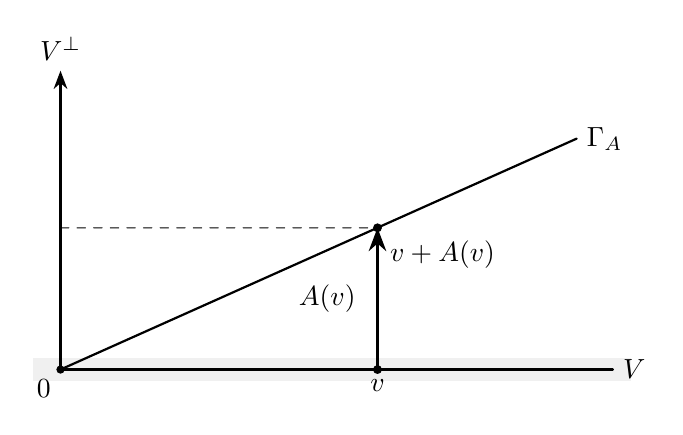
\begin{tikzpicture}[scale=1.15,>=Stealth,line join=round,line cap=round]
  % V：水平面（图中以其截线表示）
  \fill[black!6] (-0.3,-0.13) rectangle (6.3,0.13);
  \draw[thick] (0,0) -- (6.1,0) node[right] {$V$};
  % V^\perp：竖直方向
  \draw[thick,->] (0,0) -- (0,3.3) node[above] {$V^{\perp}$};
  % 原点
  \fill (0,0) circle (1.3pt) node[below left] {$0$};
  % Gamma_A：A 的图像
  \draw[thick] (0,0) -- (5.7,2.55) node[right] {$\Gamma_A$};
  % 取一点 v
  \coordinate (vb) at (3.5,0);
  \coordinate (vt) at (3.5,1.565);
  \draw[dashed,thin] (0,1.565) -- (vt);
  \draw[->,very thick] (vb) -- (vt) node[midway,left=4pt] {$A(v)$};
  \fill (vb) circle (1.4pt) node[below] {$v$};
  \fill (vt) circle (1.4pt) node[below right=1pt] {$v+A(v)$};
\end{tikzpicture}
\captionof{figure}{图像坐标 $A\mapsto\Gamma_A$。$V$ 为水平面（图中取其截线），
$V^{\perp}$ 为竖直方向，$\Gamma_A$ 是 $A$ 的图像。$A(v)$ 是点 $v$ 到
$\Gamma_A$ 的竖直位移；$A\mapsto\Gamma_A$ 因此给出
$T_V\GK\cong\Hom(V,V^{\perp})$。}
\label{fig:graph-coords}
\end{minipage}
\end{center}
则 $A\mapsto\Gamma_A$ 是 $V$ 的邻域的坐标，故
$T_V\GK\cong\Hom(V,V^{\perp})$。这些纤维同构随 $V$ 光滑变化，得到第一式；第二式
是 $\Hom(E,F)\cong E^{*}\otimes F$ 的自然同构。

Hsiang--Szczarba \cite{HsiangSzczarba1964} 的原始证明给出了同一公式的稳定版本：
若 $\xi$ 为典范丛，则
\[
  \tau(G_{N-k,k})\oplus(\xi\otimes\xi^{*})\cong N\xi_{\mathbb{R}} .
\]
在实情形用度量识别 $\xi^{*}\cong\xi$，置 $N=n+k$ 即得
\begin{equation}
  T\GK\oplus(\cG_k\otimes\cG_k)\cong(n+k)\,\cG_k .
  \label{eq:stable-tangent}
\end{equation}
这也可由 $\cG_k\oplus\cGc_k\cong\eps^{n+k}$ 与
$T\GK\cong\cG_k^{*}\otimes\cGc_k$ 直接推出。
\end{proof}

\begin{remark}
关系 \eqref{eq:stable-tangent} 是第 \ref{sec:classical} 章一切特征类计算的出发点；
它与命题 \ref{prop:tangent} 的局部形式互为补充：前者稳定、便于求总类，后者逐点、
便于看清 $\cGc_k$ 的几何来源。
\end{remark}

% ============================================================================
%  3  Stiefel--Whitney 类与欧氏嵌入障碍
% ============================================================================
\section{Stiefel--Whitney 类与欧氏嵌入障碍}
\label{sec:sw}

\subsection{Stiefel--Whitney 类与 Whitney 乘积公式}

对实向量丛 $E\to X$，其总 Stiefel--Whitney 类定义为
\begin{equation*}
  w(E)=1+w_1(E)+w_2(E)+\cdots,
\end{equation*}
其中 $w_i(E)\in H^{i}(X;\Ftwo)$，并约定 $w_0(E)=1$，且当
$i>\operatorname{rank}E$ 时 $w_i(E)=0$。Whitney 乘积公式为
$w(E\oplus F)=w(E)w(F)$；若 $E\oplus F\cong\eps^{r}$，则 $w(F)=w(E)^{-1}$。

本文反复使用下列四条规则。它们都由分裂原理得到：在适当的拉回下把丛拆成线丛的
直和，$w$ 就归约为线丛的一次类。

\begin{enumerate}[label=(\roman*),leftmargin=2.4em,itemsep=0.25em]
  \item \emph{直和}：$w(E\oplus F)=w(E)\,w(F)$，特别地 $w(\eps^{r})=1$。
  \item \emph{张量积}：若 $E$ 的形式根为 $x_1,\dots,x_k$、$F$ 的为
        $y_1,\dots,y_l$，则 $E\otimes F$ 的形式根为 $x_i+y_j$，故
        \begin{equation}
          w(E\otimes F)=\prod_{i=1}^{k}\prod_{j=1}^{l}\bigl(1+x_i+y_j\bigr).
          \label{eq:tensor}
        \end{equation}
        特别地，对线丛 $L,L'$ 有 $w_1(L\otimes L')=w_1(L)+w_1(L')$。
  \item \emph{对偶}：$E^{*}=\Hom(E,\underline{\R})$ 的形式根为 $-x_i$，而在
        $\Ftwo$ 中 $-x_i=x_i$，故 $w_i(E^{*})=w_i(E)$。
  \item \emph{$\Hom$ 丛}：$\Hom(E,F)\cong E^{*}\otimes F$，结合 (ii)(iii) 得
        其形式根同样是 $x_i+y_j$，故
        $w(\Hom(E,F))=w(E\otimes F)$。
\end{enumerate}

我们把 $w(E)^{-1}$ 的次数 $j$ 部分记作 $\wbar_j(E)$，并称 $\wbar(E)$ 为 $E$ 的
\emph{共轭 Stiefel--Whitney 类}。若 $w(E)=1+w_1+w_2+\cdots$，则在 $\Ftwo$ 上
递推得到
\begin{equation*}
  \wbar_0=1,
  \qquad
  \wbar_j=\sum_{i=1}^{j} w_i\,\wbar_{j-i}\quad (j\ge 1).
\end{equation*}
这里的共轭类是向量丛总类的逆，它与正交补丛自身的 Stiefel--Whitney 类不是同一个
对象：后者在第 \ref{sec:classical} 章记作 $v_j$。

\subsection{法丛与切丛的特征类关系}

设 $M^{d}$ 是闭光滑流形，并有光滑嵌入 $f\colon M\emb\R^{d+c}$。管状邻域定理给出
$M$ 上秩为 $c$ 的法丛 $\nu_f$，且
\begin{equation*}
  TM\oplus\nu_f\cong\eps^{d+c},
  \qquad
  w(\nu_f)=w(TM)^{-1}=\wbar(TM).
\end{equation*}
于是，秩为 $c$ 的向量丛在次数 $j>c$ 上自动没有 Stiefel--Whitney 类，即
\begin{equation*}
  \wbar_j(TM)=w_j(\nu_f)=0\quad (j>c).
\end{equation*}
换言之，若 $\wbar_j(TM)\neq0$，则 $c\ge j$。这只是一般的\emph{法丛秩障碍}；
它没有排除 $c=j$ 的临界情形。

\subsection{共轭 Stiefel--Whitney 类给出的嵌入障碍}

\begin{theorem}[法丛秩障碍]\label{thm:embedding-obstruction}
设闭光滑 $d$ 维流形 $M$ 嵌入 $\R^{d+c}$，且 $\wbar_j(TM)\neq0$，则 $c\ge j$。
特别地，若
\begin{equation}
  \delta(M)=\max\{\,j:\ \wbar_j(TM)\neq0\,\}>0,
  \label{eq:delta}
\end{equation}
则 $\embdim(M)\ge d+\delta(M)$。
\end{theorem}

\begin{proof}[证明（个人复现）]
由 $TM\oplus\nu\cong\eps^{d+c}$ 得 $w(\nu)=w(TM)^{-1}$。$\nu$ 的秩为 $c$，故
$w_j(\nu)=0$（$j>c$）。于是 $\wbar_j(TM)=w_j(\nu)\neq0$ 迫使 $j\le c$。
\end{proof}

\begin{theorem}[欧氏嵌入的临界次数判据]\label{thm:critical}
设闭光滑 $d$ 维流形 $M$ 嵌入 $\R^{d+c}$ 且 $c>0$。则
\begin{equation}
  \wbar_i(TM)=0\qquad(i\ge c).
  \label{eq:critical}
\end{equation}
因而当 $\wbar_j(TM)\neq0$ 时，实际上有 $c\ge j+1$，环境维数至少为 $d+j+1$。
\end{theorem}

\begin{proof}
设 $\nu$ 为 $M$ 的秩 $c$ 法丛。$i>c$ 时 $w_i(\nu)=0$ 已由秩给出，故只需证
$w_c(\nu)=0$。

取向量 $u\in\R^{d+c}$，使对每个 $x\in M$ 都有 $u\notin T_xM$；这样的 $u$ 一定
存在，因为 $\bigcup_{x\in M}T_xM$ 是低维子空间的并，不能充满整个空间。把常向量场
$u$ 逐点正交投影到法向，得到 $\nu$ 的一个截面 $s(x)=u-(u\text{ 的切向分量})$。
由 $u\notin T_xM$ 知 $s(x)\neq0$ 处处成立，即 $\nu$ 有处处非零的截面。

对秩为 $c$ 的实向量丛，$w_c$ 就是它的模 $2$ Euler 类；而 Euler 类是零截面与任一
横截截面的相交数（模 $2$）。既然存在处处非零的截面，该相交数为零，故
$w_c(\nu)=0$。结合秩截断得 $w_i(\nu)=0$ 对一切 $i\ge c$ 成立，再由
$w(\nu)=\wbar(TM)$ 即得 \eqref{eq:critical}。

端点上的加强正是在这一步超出秩截断：秩截断只能控制 $i>c$，而处处非零截面的存在
额外给出 $i=c$ 的消失。Oproiu 在文献 \cite[p.~177]{Oproiu1977} 中引用这一判据，
并在第 181--184 页用它排除临界环境维数。
\end{proof}

\begin{remark}[两个定理的逻辑地位]
定理 \ref{thm:embedding-obstruction} 与定理 \ref{thm:critical} 都是嵌入的
\emph{必要}条件，而非充分条件：共轭类消失并不能构造嵌入。另一方面，非浸入的
下界可以转移为嵌入的下界（嵌入必为浸入），但浸入的上界、存在性与精确值都不作此
转移。
\end{remark}

% ============================================================================
%  4  Grassmann 流形的经典非嵌入与浸入结果
%  记号约定（本文统一）：$p=s-n$ 用于 4.1 与 4.2 的下支，$m=2s-n$ 仅用于 4.2 的上支。
%  原文 4.2 用 $p=2s-n$、$q=s-n$，与 4.1 的 $p=s-n$ 冲突，故改写如上。
% ============================================================================
\section{Grassmann 流形的经典非嵌入与浸入结果}
\label{sec:classical}

\subsection{Oproiu 关于 $G_{2,n}$ 的结果}

\begin{theorem}[Oproiu，原文定理 1]\label{thm:oproiu-G2}
除原文排除的低维情形 $G_{2,1}\cong\R P^{2}$ 外，令 $s=2^{r}$ 为严格大于 $n$ 的
最小二进制幂，即 $2^{r-1}\le n<s$。
\begin{enumerate}[label=(\roman*),leftmargin=2.2em]
  \item 若 $n\neq s-1$，则
        \[
          G_{2,n}\nemb\R^{2s-2},
          \qquad
          G_{2,n}\not\imm\R^{2s-3};
        \]
  \item 若 $n=s-1$，则
        \[
          G_{2,s-1}\nemb\R^{3s-2},
          \qquad
          G_{2,s-1}\not\imm\R^{3s-3}.
        \]
\end{enumerate}
\end{theorem}

原文还给出相应的 Whitney 型正结果；以下只讨论非嵌入的证明。

\begin{proof}[证明复现]
设 $w=1+w_1+w_2=w(\cG_2)$。按张量积公式 \eqref{eq:tensor}，若 $\cG_2$ 的形式根
为 $x_1,x_2$，则 $\cG_2\otimes\cG_2$ 的根为 $x_i+x_j$，其中
$x_1+x_1=x_2+x_2=0$、$x_1+x_2=w_1$，故
$w(\cG_2\otimes\cG_2)=(1+w_1)^{2}$。代入 \eqref{eq:stable-tangent} 得
\begin{equation*}
  w(TG_{2,n})\,(1+w_1)^{2}=w^{n+2},
  \qquad
  \wbar(TG_{2,n})=(1+w_1)^{2}\,w^{-(n+2)} .
\end{equation*}
因为 $w^{2s}=1$（其所有正次数分量的次数都超过 $\dim G_{2,n}=2n$），所以
\begin{equation}
  \wbar(TG_{2,n})=(1+w_1)^{2}\,w^{2s-n-2}. \label{eq:wbar-G2}
\end{equation}
这里的等式在真实上同调商环中成立。

设 $n\le s-2$。Oproiu 的 Schubert 计算给出 $w^{s}=1$；令 $p=s-n\ge2$，则
\begin{equation*}
  \wbar=(1+w_1)^{2}w^{p-2},
  \qquad
  \wbar_{2p-2}=w_1^{2}w_2^{p-2}.
\end{equation*}
Schubert 乘法给出
\begin{equation}
  w_1^{2}w_2^{p-2}=(p-1,p-1)+(p-2,p)\neq0. \label{eq:schubert-G2}
\end{equation}
两项是加法基中不同的 Schubert 类，且 $p\le s/2$ 保证它们合法，故真实商环中的非零
性已经得到。此时 $d=2n=2s-2p$，非零次数为 $j=2p-2$，有 $d+j=2s-2$。由定理
\ref{thm:critical} 排除临界嵌入 $\R^{2s-2}$；由定理
\ref{thm:embedding-obstruction} 排除余维 $j-1$ 的浸入环境 $\R^{2s-3}$。

边界 $n=s-1$ 不能代入 $p-2$。由 \eqref{eq:wbar-G2} 直接取指数 $s-1$，其次数 $s$
部分满足
\begin{equation}
  \wbar_s=(1,s-1)+\text{其他 Schubert 类}\neq0. \label{eq:wbar-boundary}
\end{equation}
为核对系数，展开 $(1+w_1)^{2}w^{s-1}$：在 $w_1^{s-2i}w_2^{i}$ 中系数为
$\binom{s+1-i}{i+1}$；$i=0$ 给出 $w_1^{s}$，其中 $(1,s-1)$ 的系数为 $1$；对
$s\ge4$，$i=1$ 的系数 $\binom{s}{2}$ 为偶数，而 $i\ge2$ 的 Schubert 展开第一坐标
至少为 $2$，故该基元素不被抵消。由于 $d=2s-2$，定理 \ref{thm:critical} 排除
$\R^{3s-2}$，定理 \ref{thm:embedding-obstruction} 排除 $\R^{3s-3}$ 的浸入。
\end{proof}

\begin{remark}
以上是 Oproiu 原文定理 1 的嵌入／浸入分层复现；其临界嵌入端点依赖定理
\ref{thm:critical}，而不是单独的秩截断。
\end{remark}

\subsection{Oproiu 关于 $G_{3,n}$ 的结果}

\begin{theorem}[Oproiu，原文定理 2]\label{thm:oproiu-G3}
令 $s=2^{r}$ 满足 $2s<3n<4s$，且 $n\ge3$。则
\begin{enumerate}[label=(\alph*),leftmargin=2.2em]
  \item 当 $\tfrac23s<n\le s-3$ 时，$G_{3,n}\nemb\R^{3s-3}$；
  \item 当 $n=s-2$ 时，$G_{3,s-2}\nemb\R^{4s-3}$；当 $n=s-1$ 且 $s\ge8$ 时，
        $G_{3,s-1}\nemb\R^{5s-3}$；
  \item 当 $s\le n<\tfrac43s$ 时，$G_{3,n}\nemb\R^{6s-3}$；
  \item 另有独立的小参数结论 $G_{3,3}\nemb\R^{15}$。
\end{enumerate}
\end{theorem}

\begin{proof}[证明复现]
令 $w=1+w_1+w_2+w_3$，并置
\begin{equation*}
  A=(1+w_1)(1+w_1+w_2)+w_3=1+w_1^{2}+w_2+w_1w_2+w_3 .
\end{equation*}
由 \eqref{eq:stable-tangent} 与张量积公式，
\begin{equation*}
  w(TG_{3,n})\,A^{2}=w^{n+3}.
\end{equation*}
由于 $4s>3n=\dim G_{3,n}$，有 $w^{4s}=1$，从而
\begin{equation}
  \wbar=A^{2}\,w^{4s-n-3}. \label{eq:wbar-G3}
\end{equation}

在上支 $s\le n<\tfrac43s$，Oproiu 的 Schubert 引理给出 $w^{2s}=1$。令
$m=2s-n$，则
\begin{equation*}
  \wbar=A^{2}w^{m-3},
  \qquad
  \wbar_{3m-3}=(w_1^{2}w_2^{2}+w_3^{2})\,w_3^{m-3}.
\end{equation*}
其 Schubert 展开含四个不同的基元素
\begin{equation*}
  (m-3,m-1,m+1)+(m-3,m,m)+(m-2,m-2,m+1)+(m-1,m-1,m-1),
\end{equation*}
最后一项在 $m-1\le n$ 时合法，故该类非零。于是 $3n+(3m-3)=6s-3$，由定理
\ref{thm:critical} 排除该环境维数。

在下支 $\tfrac23s<n\le s-3$，令 $p=s-n\ge3$。此时 $w^{s}=1$，
\eqref{eq:wbar-G3} 化为 $\wbar=A^{2}w^{p-3}$，同样得到
\begin{equation*}
  \wbar_{3p-3}\neq0,
\end{equation*}
且 $3n+(3p-3)=3s-3$，从而排除 $\R^{3s-3}$。两支的非零性均在 Schubert 加法基中
判定，而不是自由多项式中的形式非零。

边界由 Oproiu 的引理 4 单独处理：当 $n=s-2$ 时，$\wbar_{s+3}$ 的展开含关键基
元素 $(1,4,s-2)$；当 $n=s-1$ 时，$\wbar_{2s}$ 的展开含 $(2,s-1,s-1)$。它们分别
给出
\begin{equation*}
  3(s-2)+(s+3)=4s-3,
  \qquad
  3(s-1)+2s=5s-3 .
\end{equation*}
小参数 $G_{3,3}\nemb\R^{15}$ 是原文另行直接计算的结论，不由上述分支外推。
\end{proof}

\begin{remark}
以上均为 Oproiu 已知定理的复现，不是新的非嵌入定理。$n=s-2$ 这一支的具体数值
核对见第 \ref{sec:G36} 节。
\end{remark}

\subsection{Hiller--Stong 的浸入维数结果}

本节只陈述与本文主线有关的浸入维数结论，并一律以「Hiller--Stong 命题 $m.n$」
的形式引用原文编号，以免与本文自身的编号混淆。

\paragraph{Lam 型上界。}
对 $G_k(\R^{n+k})$，Lam 的估计为
\begin{equation*}
  \imdim\bigl(G_k(\R^{n+k})\bigr)\le\binom{n+k}{2},
\end{equation*}
其证明使用 $\cG_k\oplus\cG_n\cong(n+k)\eps$ 并施加第二外幂函子，得到切丛的一个
平凡补，再由 Hirsch 的浸入定理得到浸入。这是 immersion 的上界。

\paragraph{命题 4.1 与未编号的推论。}
Hiller--Stong 命题 4.1：若 $k\le2^{s}\le n$ 且 $n+k\le2^{s+1}$，则
\begin{equation*}
  \imdim\bigl(G_k(\R^{n+k})\bigr)\ge k\,(2^{s+1}-1).
\end{equation*}
其后紧接一条未编号的 \emph{Corollary}：当 $n=2^{s}$ 时，
\begin{equation*}
  \binom{2^{s}+k}{2}\ \ge\ \imdim\bigl(G_k(\R^{2^{s}+k})\bigr)\ \ge\
  \binom{2^{s}+k}{2}-\binom{2^{s}-k}{2}=k\,(2^{s+1}-1).
\end{equation*}
另一方面，Whitney 型估计给出 $\imdim\le2\dim M-1$，即
$\imdim(G_k(\R^{2^{s}+k}))\le2^{s+1}k-1$。这一上界与上式的左端
$\binom{2^{s}+k}{2}$ 一般并不相同，两组上界应分别记录，或取其中较小者，不宜
合并写成一个「双侧夹逼」。

\paragraph{命题 4.2 与命题 4.3。}
命题 4.2：若 $k\le n=2^{s}-1$，则
\begin{equation*}
  \imdim\bigl(G_k(\R^{n+k})\bigr)\ \ge\
  \binom{n+k}{2}-\binom{2^{s}-k}{2}.
\end{equation*}
命题 4.3：若 $k\le2^{s}-1$ 且 $n+k=2^{s+1}+1$，则共轭类的最高非零次数为
\begin{equation*}
  \delta=k(k-1)+(n-1),
\end{equation*}
由此得到相应的 immersion 下界。

\paragraph{引言的精确等式。}
文章引言还给出 $\imdim(G_k(\R^{2k}))=k(2k-1)$ 以及相邻奇维情形的精确等式；这些
等式仍然只属于 immersion。

\begin{remark}
以上均为已核验的浸入维数结果。非浸入的下界可以作为嵌入的下界（嵌入必为浸入），
但浸入的存在性、上界与精确值都不能自动转成嵌入的相应结论。
\end{remark}

% ============================================================================
%  5  计算实例与讨论
%  记号：$v_j=w_j(\cGc_k)$ 专指正交补丛自身的类；$\wbar_j$ 专指总类之逆。
% ============================================================================
\section{计算实例与讨论}

\subsection{切丛类的计算方法}

本文的计算统一在真实的上同调环
\begin{equation*}
  H^{*}(\GK;\Ftwo)\cong\Ftwo[w_1,\dots,w_k]/I_{k,n}
\end{equation*}
中进行，其中 $I_{k,n}$ 由 $w(\cG_k)\,w(\cGc_k)=1$ 中次数高于补丛秩的分量生成。
计算时先在自由多项式环中递推求出总类或其逆总类，随后必须按 $I_{k,n}$ 约化；
自由多项式中的非零并不等于上同调环中的非零。

由 \eqref{eq:stable-tangent} 与度量同构，
\begin{equation*}
  \wbar(T\GK)=w(\cG_k\otimes\cG_k)\,w(\cG_k)^{-(n+k)}
\end{equation*}
是在商环中成立的等式。若 $x_1,\dots,x_k$ 是 $\cG_k$ 的形式 Stiefel--Whitney 根，
则
\begin{equation*}
  w(\cG_k\otimes\cG_k)=\prod_{i<j}\bigl(1+(x_i+x_j)^{2}\bigr),
\end{equation*}
因为 $i=j$ 时对应的根为 $x_i+x_i=0$，而每个 $i<j$ 的根出现两次，给出平方因子。
实际计算时仍须把得到的对称多项式写回 $w_1,\dots,w_k$，并在
$H^{*}(\GK;\Ftwo)$ 中约化。

\subsection{代表性参数实例}

\begin{example}[$G_{2,2}=G_2(\R^{4})$]\label{ex:G22}
令 $w_i=w_i(\cG_2)$，并以 $v_j=w_j(\cGc_2)$ 记正交补丛自身的类。由补丛秩为 $2$，
\begin{equation*}
  (1+w_1+w_2)\,(1+v_1+v_2+v_3+\cdots)=1,
\end{equation*}
且 $v_j=0$ 对 $j>2$ 成立。形式递推给出 $v_1=w_1$、$v_2=w_1^{2}+w_2$；而
$v_3=w_1^{3}$ 恰是补丛秩为 $2$ 所强加的关系，即商环中 $w_1^{3}=0$，故 $v_3=0$。
于是
\begin{equation*}
  I_{2,2}=\bigl(w_1^{3},\ w_1^{4}+w_1^{2}w_2+w_2^{2}\bigr).
\end{equation*}
另一方面，\eqref{eq:stable-tangent} 给出
$TG_{2,2}\oplus(\cG_2\otimes\cG_2)\cong4\cG_2$。在模 $2$ 特征类中
$w(\cG_2\otimes\cG_2)=(1+w_1)^{2}=1+w_1^{2}$，而
\begin{equation*}
  (1+w_1+w_2)^{4}=1+w_1^{4}+w_2^{4}=1
\end{equation*}
在上述商环中成立（次数超过 $\dim G_{2,2}=4$ 的项自动为零，且关系消去
$w_1^{4}$）。故 $w(TG_{2,2})=1+w_1^{2}$，$\wbar(TG_{2,2})=1+w_1^{2}$。

在标准单项式基中 $w_1^{2}\neq0$，所以 $\wbar_2(TG_{2,2})\neq0$，并由各高次类
消失得 $\delta(G_{2,2})=2$。定理 \ref{thm:embedding-obstruction} 给出法丛余维
$c\ge2$，从而 $G_{2,2}$ 不能嵌入 $\R^{5}$。这里只用到秩截断；Oproiu 定理
\ref{thm:oproiu-G2} 对 $s=4,n=2$ 还用定理 \ref{thm:critical} 排除了 $\R^{6}$。
\end{example}

\subsection{固定 $k$ 时的数值现象}

本文核验了 Hiller--Stong 原文第 4 节的命题 4.1、其后未编号的 \emph{Corollary}、
命题 4.2 与命题 4.3。原文并未给出「Corollary 4.1」这一编号，因此本文不使用该
名称。准确的说法是：当 $k\le n=2^{s}$ 时，该 \emph{Corollary} 给出
\begin{equation*}
  \binom{2^{s}+k}{2}\ \ge\ \imdim\bigl(G_k(\R^{2^{s}+k})\bigr)\ \ge\
  \binom{2^{s}+k}{2}-\binom{2^{s}-k}{2}=k\,(2^{s+1}-1),
\end{equation*}
而 Whitney 型估计给出 $\imdim\le2^{s+1}k-1$。两个上界一般不同，故不把它们写成
同一个「双侧夹逼」。命题 4.2 与 4.3 分别处理 $n=2^{s}-1$ 与 $n+k=2^{s+1}+1$ 的
参数情形。这里的 $\imdim$ 始终是浸入维数，不能把这些「平台」现象转写为嵌入维数
结论。本文所列固定 $k$ 的计算均标为文献下界或个人复现，不存在完整证明的模式不外推
为新定理。

\subsection{特征类障碍的方法边界}

本文实际使用两种必要条件。第一种是\emph{法丛秩条件}：若 $M^{d}$ 嵌入
$\R^{d+c}$，则 $w_j(\nu)=0$ 对 $j>c$，从而 $\wbar_j(TM)\neq0$ 只推出 $c\ge j$。
这一论证只依赖 $TM\oplus\nu\cong\eps^{d+c}$ 与向量丛的秩，不需要知道法丛的具体
几何构造。第二种是定理 \ref{thm:critical} 的临界次数判据，它把结论加强为
$c\ge j+1$。

两种条件都不是充分条件：共轭类全部消失只说明这一组模 $2$ 特征类不再排除某个
余维，它既不能构造嵌入，也不能保证候选浸入的全局单射性。因此 Hiller--Stong 的
浸入维数下界必须留在浸入问题的语境中。

此外，「形式非零」也不是充分证据。对 $\GK$，必须先在
$H^{*}(\GK;\Ftwo)$ 中约化，再用 Schubert 类或 Gr\"obner 标准单项式判定非零性。
Oproiu 的证明正是通过 Schubert 乘法确认关键项没有抵消。故本文把「公式推导」
「商环中的非零性」「由非零性得到的排除」列为三个必须分别核查的步骤。

\subsection{Oproiu 与 Hiller--Stong 的结果对照}

下表只比较研究对象与逻辑地位，不把两篇论文的维数公式拼接成新的统一定理。设
$d=\dim\GK=kn$，$c=N-d$ 为余维。

\begin{table}[!htbp]
\centering
\footnotesize
\renewcommand{\arraystretch}{1.18}
\caption{Oproiu 与 Hiller--Stong 的研究对象及逻辑地位对照}
\label{tab:comparison}
\begin{tabularx}{\textwidth}{@{}>{\raggedright\arraybackslash}p{2.45cm}
    >{\raggedright\arraybackslash}p{2.95cm}
    >{\raggedright\arraybackslash}X
    >{\raggedright\arraybackslash}X
    >{\raggedright\arraybackslash}p{2.45cm}@{}}
\toprule
来源与工具 & 研究对象 & 典型输入 & 直接得到的结论 & 本文中的定位 \\
\midrule
Oproiu（1977），定理 1--2 & embedding；定理 1 另列 immersion &
$\wbar_j$ 的 Schubert 非零性；二进制参数分段 &
排除指定的 $\R^{N}$，并在定理 1 中同时排除一个低一维的浸入环境 &
第 \ref{sec:classical} 章的已核验非嵌入定理 \\
\addlinespace[2pt]
本文定理 \ref{thm:embedding-obstruction} & embedding &
$TM\oplus\nu\cong\eps^{d+c}$ 与秩截断 &
$\wbar_j\neq0\Rightarrow c\ge j$，即排除 $\R^{d+j-1}$ &
一般法丛秩障碍；必要而非充分 \\
\addlinespace[2pt]
本文定理 \ref{thm:critical} & embedding &
额外使用 $w_c(\nu)=0$（Thom 类） &
$\wbar_j\neq0\Rightarrow c\ge j+1$，即排除 $\R^{d+j}$ &
解释定理 \ref{thm:oproiu-G2} 的嵌入端点 \\
\addlinespace[2pt]
Hiller--Stong（1981） & immersion &
稳定切丛、模 $2$ 特征类 & 给出 $\imdim$ 的下界或精确值 &
第 4.3 节的浸入维数结果，不改写为 embedding \\
\bottomrule
\end{tabularx}
\end{table}

因此，不能仅凭「同一个共轭类出现于两篇论文」就比较两者的环境维数大小：Oproiu
的结论依赖嵌入的临界次数条件，而 Hiller--Stong 的主对象是浸入维数。只有先固定
研究对象、参数范围与余维定义，比较才有意义。

\FloatBarrier

\subsection{Hiller（1980）：上同调环、旗流形检测与递归约化}
\label{sec:hiller1980}

\begin{remark*}[文献核验状态]
H.~L.~Hiller, \emph{On the Cohomology of Real Grassmanians}, Transactions of
the American Mathematical Society \textbf{257} (1980), no.~2, 521--533,
DOI: 10.1090/S0002-9947-1980-0552272-2 \cite{Hiller1980}。本文依据原始 PDF 核对
原文第 521--533 页的编号结果。该文的研究对象是
$H^{*}(G_k(\R^{n+k});\Ftwo)$ 中的 Schubert calculus、$w_1$ 的高度与
Lusternik--Schnirelmann category；它提供非零性计算的上同调基础，本身不给出
嵌入维数或浸入维数。
\end{remark*}

\paragraph{乘法公式的出处。}
Oproiu 原文第 180 页引用 S.~S.~Chern 的 Schubert 乘法公式，并在引理 1--4 中给出
本文所需的具体展开；Hiller--Stong \cite{HillerStong1981} 第 363--365 页给出完全
旗流形投影、拉回单射、顶维单项式检测与法丛总类公式的可复核框架。本文把 Hiller
（1980）定位为 Borel 商环与递归约化的直接来源，把 Oproiu 与 Hiller--Stong 定位为
Schubert／旗流形非零性的核验来源。

\begin{theorem}[Borel 表示，Hiller 原文 Theorem 1.1(i)]\label{thm:borel}
令 $u_i=w_i(\cG_k)$，$v_j=w_j(\cGc_k)$，其中 $1\le i\le k$、$1\le j\le n$。则
\begin{equation*}
  H^{*}(\GK;\Ftwo)\cong
  \Ftwo[u_1,\dots,u_k,v_1,\dots,v_n]\big/\,I_{k,n},
\end{equation*}
其中 $I_{k,n}$ 由 $(1+u_1+\cdots+u_k)(1+v_1+\cdots+v_n)=1$ 的齐次分量生成。
Hiller 称 $v_j$ 为 universal bundle 的 normal Stiefel--Whitney classes；本文
沿用记号 $v_j=w_j(\cGc_k)$。消去 $v_j$ 后得到只含 $u_1,\dots,u_k$ 的商环，这正是
本文进行 Gr\"obner 约化与 Schubert 非零性判定时所用的真实上同调环。
\end{theorem}

\begin{theorem}[旗流形计算，Hiller 原文 \textsection2 与式 (2.1)]\label{thm:flag}
对完全旗流形投影（Hiller 原文记作 $\rho$，本文统一记作 $\pi$）
\begin{equation*}
  \pi\colon\Flag(\R^{n+k})\longrightarrow \GK,
\end{equation*}
诱导映射 $\pi^{*}$ 在上同调上是单射。若 $e_1,\dots,e_{n+k}$ 是旗流形上的一维类，
则
\begin{equation*}
  \pi^{*}(u_i)=\sigma_i(e_1,\dots,e_k),
  \qquad
  \pi^{*}(v_j)=\sigma_j(e_{k+1},\dots,e_{k+n}),
\end{equation*}
其中 $\sigma_i$ 表示初等对称函数。
\end{theorem}

Hiller 的证明把 Grassmann 流形上的关系转移到完全旗流形的 coinvariant ring 中；
因此要证明某个类非零，可以先利用 $\pi^{*}$ 的单射性检查其拉回。这与
Hiller--Stong 所使用的检测框架相互印证，也解释了 Oproiu 证明中 Schubert 非零性
步骤的代数背景。

\begin{proposition}[Hiller 原文 Proposition 2.2 的直接应用]\label{prop:hiller22}
若 $n+k=2^{s}$，则在 $H^{*}(\GK;\Ftwo)$ 中 $u_1^{2^{s}}=0$。
\end{proposition}

\begin{proof}
由定理 \ref{thm:flag}，$\pi^{*}(u_1)=e_1+\cdots+e_k$。在特征 $2$ 中 Frobenius
恒等式给出 $\pi^{*}(u_1^{2^{s}})=e_1^{2^{s}}+\cdots+e_k^{2^{s}}$。Hiller 利用
完全旗流形上对称函数理想的基本多项式关系说明右端属于该理想，故拉回为零；由于
$\pi^{*}$ 单射，原类即为零。
\end{proof}

\paragraph{附录的递归约化。}
Hiller 进一步消去 normal classes，得到只含 $u_1,\dots,u_k$ 的理想 $J(k,n)$。
对 $k=2$，记两个递归关系为 $f_n=f_{1,n}$、$g_n=f_{2,n}$，附录给出
\begin{equation*}
  f_{n+1}=u_1f_n+g_n,
  \qquad
  g_{n+1}=u_2f_n,
\end{equation*}
并以 $f_n=g_n=0$ 生成 $J(2,n)$。特别地，附录 Proposition 5 证明：若
$n=(2^{s}-1)+d$ 且 $0\le d<2^{s}$，则
\begin{equation*}
  u_2^{n}+u_1^{2(2^{s}-1)}u_2^{d}=0,
  \qquad\text{且}\qquad
  u_1^{2(2^{s}-1)}u_2^{d}\neq0;
\end{equation*}
附录 Proposition 6 还在同一参数范围下给出 $u_1^{2^{s+1}-1}=0$。

\begin{remark}
Hiller（1980）为第 5.1 节的商环表示、例 \ref{ex:G22} 的 Gr\"obner 基与第
\ref{sec:stong} 节的旗流形非零性提供了直接出处。本文把 Hiller 的结果定位为上
同调与计算工具；Oproiu 的非嵌入结论仍由 Oproiu 原文给出，Hiller--Stong 的结论仍
严格属于 immersion。
\end{remark}

\subsection{Hiller 递归理想与 $G_{2,n}$ 的小参数约化}
\label{sec:recursion}

本节把 Hiller（1980）的 Borel 商环递归与第 5.2 节的计算逐项对照，并补充
$G_{2,3}$ 的手工约化。目标是核对计算机制，而不是提出新的 Gr\"obner 基结果；
所有等式均在 $\Ftwo[u_1,u_2]$ 的上同调商环中解释。

令 $u_i=w_i(\cG_2)$，以形式变量 $t$ 记
\begin{equation*}
  \frac{1}{1+u_1t+u_2t^{2}}=\sum_{r\ge0} f_r t^{r},
  \qquad
  f_0=1,\quad f_1=u_1,\quad f_r=u_1f_{r-1}+u_2f_{r-2}\ (r\ge2).
\end{equation*}
在 $G_{2,n}$ 上正交补丛的秩为 $n$，故 Borel 关系等价于令 $f_{n+1},f_{n+2}$ 为零，
更高的 $f_r$ 随之归零。因此
\begin{equation*}
  H^{*}(G_{2,n};\Ftwo)\cong\Ftwo[u_1,u_2]\big/\,(f_{n+1},f_{n+2}),
\end{equation*}
这正是第 5.2 节由补丛高次类得到的关系理想。

\begin{example}[$G_{2,2}$ 的逐项对照]\label{ex:G22-grobner}
递推给出 $f_3=u_1^{3}$、$f_4=u_1^{4}+u_1^{2}u_2+u_2^{2}$，故
$I_{2,2}=(u_1^{3},\,u_1^{4}+u_1^{2}u_2+u_2^{2})$。用分次字典序 $u_1>u_2$ 做模
$2$ 的 Buchberger 约化：先以 $u_1^{3}$ 约去第二个生成元中的 $u_1^{4}$，得
$u_1^{2}u_2+u_2^{2}$；继续处理相应的 $S$-多项式，得到
\begin{equation*}
  \mathcal{G}_{2,2}=\bigl\{\,u_1^{3},\ u_1^{2}u_2+u_2^{2},\ u_1u_2^{2},\
  u_2^{3}\,\bigr\}.
\end{equation*}
标准单项式为 $1,u_1,u_1^{2},u_2,u_1u_2,u_2^{2}$，恰六个，与
$G_2(\R^{4})$ 的模 $2$ Schubert 细胞数一致。特别地 $u_1^{2}$ 未被约化为零，这与
例 \ref{ex:G22} 中 $\wbar_2(TG_{2,2})=u_1^{2}\neq0$ 一致。
\end{example}

\begin{example}[$G_{2,3}$ 的附加交叉检查]\label{ex:G23}
继续递推得 $f_4=u_1^{4}+u_1^{2}u_2+u_2^{2}$、$f_5=u_1^{5}+u_1u_2^{2}$。由
$u_1f_4+f_5$ 得 $u_1^{3}u_2$；随后的 $S$-多项式给出 $u_1^{2}u_2^{2}+u_2^{3}$、
$u_1u_2^{3}$、$u_2^{4}$。因此可取
\begin{equation*}
  \mathcal{G}_{2,3}=\bigl\{\,u_1^{4}+u_1^{2}u_2+u_2^{2},\ u_1^{3}u_2,\
  u_1^{2}u_2^{2}+u_2^{3},\ u_1u_2^{3},\ u_2^{4}\,\bigr\},
\end{equation*}
其首项为 $u_1^{4},u_1^{3}u_2,u_1^{2}u_2^{2},u_1u_2^{3},u_2^{4}$。故标准单项式总数
为 $10=\binom{5}{2}$，与 $G_2(\R^{5})$ 的 Schubert 细胞数相符。
\end{example}

\begin{remark}
递归理想把「补丛高次类消失」转化为可执行的商环约化；$G_{2,2}$ 是其最小实例，
$G_{2,3}$ 显示了额外 $S$-多项式如何产生有限维标准单项式空间。上述计算属于个人
复现，未声称新的 Gr\"obner 基定理。
\end{remark}

\subsection{Stong（1982）：旗流形评价与杯积的交叉核验}
\label{sec:stong}

\begin{remark*}[文献核验状态]
R.~E. Stong, \emph{Cup Products in Grassmannians}, Topology and its
Applications \textbf{13} (1982), 103--113 \cite{Stong1982}。本文直接读取原文，
将其定位为上同调非零性与杯积的来源，不改写为欧氏嵌入定理。
\end{remark*}

Stong 使用 Borel 商环与完全旗流形投影
$\pi\colon\Flag(\R^{n+k})\to G_k(\R^{n+k})$，证明 $\pi^{*}$ 单射，并以旗流形
顶维评价检测 Grassmann 流形上的非零杯积。

\paragraph{$w_1$ 的高度。}
当 $2\le k\le n$ 且 $2^{s}<n+k\le2^{s+1}$ 时，Stong 给出
\begin{equation*}
  \operatorname{height}(w_1)=
  \begin{cases}
    2^{s+1}-2, & k=2,\ \text{或}\ k=3\ \text{且}\ n+k=2^{s}+1,\\[2pt]
    2^{s+1}-1, & \text{其他情形}.
  \end{cases}
\end{equation*}
这只是典范丛类的杯积信息，不能替代切丛共轭类 $\wbar_j(T\GK)$ 的计算。

\paragraph{一个顶维杯积。}
对 $s\ge2$，在 $G_3(\R^{2^{s}+2})=G_{3,2^{s}-1}$ 的顶维中有
\begin{equation*}
  w_1^{2^{s+1}-1}w_2^{2^{s-1}-1}\neq0,
\end{equation*}
其次数为 $3\cdot2^{s}-3$，恰等于流形维数；特别地 $s=2$ 给出 $G_{3,3}$ 中
$w_1^{7}w_2\neq0$。这仍然是典范丛的杯积，与切丛的共轭类不是同一个对象。

\paragraph{旗流形评价原则。}
若 $e_1,\dots,e_{n+k}$ 是完全旗流形上的一维类，则
$\pi^{*}(w_i)=\sigma_i(e_1,\dots,e_k)$ 且 $\pi^{*}$ 单射；旗流形顶维中，指数为
$0,1,\dots,n+k-1$ 的单项式评价为 $1$。因此，把拉回后的类乘以互补单项式并检查
顶维系数是否为 $1$，即可判定 Grassmann 流形上该类的非零性。这条原则与第
\ref{sec:hiller1980} 节的技术一致，是全文判定「商环中非零」的统一依据。

\paragraph{与切丛公式的联系。}
Stong 还使用同 $k$ 的嵌入
\begin{equation*}
  G_k(\R^{n+k-1})\subset G_k(\R^{n+k}),
\end{equation*}
其法丛为 $\cG_k$（此处必须保持 $k$ 不变）。限制切丛的分解为
$TG_k(\R^{n+k-1})\oplus\cG_k$，与第 \ref{sec:geometry} 节的公式相容。

\subsection{$G_{3,6}$：边界分支的手工核对}
\label{sec:G36}

取 $n=6$，则 $s=8$ 且 $n=s-2$。因此 $\dim G_{3,6}=18$，Oproiu 的边界分支要求
核对
\begin{equation*}
  \wbar_{s+3}(TG_{3,6})=\wbar_{11}(TG_{3,6})\neq0 .
\end{equation*}
引理 4 给出的关键 Schubert 基元素是 $(1,4,s-2)=(1,4,6)$，其次数为
$1+4+6=11$，合法性为 $0\le1\le4\le6\le n=6$。

为独立核对，令 $h_0=1$、$h_j=0$（$j<0$），并在 $G_{3,6}$ 中递推
\begin{equation*}
  h_j=w_1h_{j-1}+w_2h_{j-2}+w_3h_{j-3};
\end{equation*}
相应的 Borel 关系为 $h_7=h_8=h_9=0$。由 Jacobi--Trudi 行列式，该 Schubert 类可
写成
\begin{equation*}
  (1,4,6)=(w_1h_4+h_5)\,h_6 .
\end{equation*}
在次数 $11$ 的单项式空间中，把 $h_7,h_8,h_9$ 的所有齐次倍数作为关系，模 $2$
线性消元得到关系秩 $9$；再加入 $(w_1h_4+h_5)h_6$ 后秩为 $10$。因此该类在商环中
确实非零——这一判定是在商环中完成的，不在自由多项式环中。

由定理 \ref{thm:critical}，$\wbar_{11}\neq0$ 排除临界环境
$\R^{18+11}=\R^{29}=\R^{4s-3}$；若只用秩截断，则只能排除余维小于 $11$ 的环境。
两者相比，端点的额外作用一目了然。

% ============================================================================
%  6  总结与进一步问题
% ============================================================================
\section{总结与进一步的问题}

本文围绕「典范丛——切丛——法丛——共轭 Stiefel--Whitney 类」这条线索，为实
Grassmann 流形的欧氏非嵌入问题建立了一条统一的分析链。对
$\GK=G_k(\R^{k+n})$，典范分解 $\cG_k\oplus\cGc_k\cong\eps^{k+n}$ 与切丛公式
\begin{equation*}
  T\GK\cong\Hom(\cG_k,\cGc_k)
\end{equation*}
把几何问题转化为向量丛特征类的计算问题。若 $M^{d}$ 嵌入 $\R^{d+c}$，则法丛满足
$w(\nu)=w(TM)^{-1}$，非零的共轭类 $\wbar_j(TM)$ 至少迫使 $c\ge j$；再调用欧氏
嵌入的临界次数判据（定理 \ref{thm:critical}），可排除 $c=j$ 的端点。这两条都是
嵌入的\emph{必要}条件，而且由于嵌入包含全局单射性，它们不能替代对嵌入本身的
构造。

本文核验并复现了两类文献结果。第一类是 Oproiu 关于 $G_{2,n}$ 与 $G_{3,n}$ 的
非嵌入定理：其二进制参数分段、稳定切丛公式以及关键 Schubert 类的非零性，都必须
在真实的 Grassmann 上同调环中理解；尤其要把临界次数判据与一般的秩截断分开。
第二类是 Hiller--Stong 的浸入维数结果：Lam 型上界、命题 4.1、未编号的
\emph{Corollary}、命题 4.2 与命题 4.3 说明模 $2$ 特征类可以给出一系列 immersion
下界，并须注意它们与 Whitney 型上界并不是同一个数。这两类结论的研究对象不同
——前者是 embedding，后者是 immersion——不能互相替代。

本文的个人复现包括：Grassmann 切丛公式的局部图像证明、法丛秩障碍定理、
$G_{2,2}$ 的商环与 Gr\"obner 标准单项式检查、$G_{2,3}$ 的附加交叉检查，以及
$G_{3,6}$ 边界类的商环秩核验。这些复现的价值在于把「形式展开——商环约化——
非零性判定——维数排除」四个步骤分开检查；它们不构成新的非嵌入定理。凡缺乏一般
证明的固定参数计算，本文只标为文献结果或个人复现，不外推为定理。

归结起来，全文的逻辑层级是清楚的。第一层是向量丛结构：局部图像坐标给出
$T\GK\cong\Hom(\cG_k,\cGc_k)$。第二层是法丛的必要条件：秩截断给 $c\ge j$，
临界次数判据把它加强为 $c\ge j+1$。第三层是具体参数族的计算：Oproiu 用二进制
分段与 Schubert 非零性得到非嵌入结论，Hiller--Stong 用稳定切丛与模 $2$ 计算得到
浸入维数下界。第四层是可复现性：Hiller、Hiller--Stong 与 Stong 的商环、旗流形
方法说明，任何「非零」断言都必须在真实的 Grassmann 上同调商环中完成约化与评价。
本文没有把特征类公式包装成「最小嵌入维数已求出」的强结论；特征类给出必要条件，
文献的 Schubert／旗流形计算把必要条件落实到参数族，而嵌入的构造或更精细的排除
属于另一个问题。

后续工作仍有两项。其一，对第 \ref{sec:classical} 章 $G_{3,n}$ 的边界参数与第 5 章
的代表性计算做独立的商环复核，避免把自由多项式中的形式非零当成上同调类非零。
其二，在明确标注「探索性观察」的前提下，对 $G_{2,n}$ 的共轭类做有限参数实验，
并与 Oproiu 的参数族逐项比较；在完成文献查重与严格证明之前，不宣称新的闭式
定理。

综上，Stiefel--Whitney 类方法适合提供可靠的非嵌入必要条件与浸入维数下界，但
通常不能单独决定最小嵌入维数。后续研究应保持三条边界：在真实上同调商环中计算；
在引用中给出准确的定理编号与参数范围；始终分开书写 embedding、immersion 与
其他受限嵌入问题。


\appendix
\clearpage
% ============================================================================
%  附录 A：证据层级与核验状态
% ============================================================================
\section{证据层级与核验状态}
\label{app:log}

正文中的结论分为三类：带原始文献与编号的已知定理、标注为「个人复现」的自算内容、
以及仅保留在方法边界中的未推广模式。下表把正文用到的每个来源与其证据强度对齐；
研究过程的日志与附件访问记录不进入正文，仅保留在本节末尾。

\begin{table}[!htbp]
\centering
\footnotesize
\renewcommand{\arraystretch}{1.22}
\caption{来源与核验状态}
\label{tab:status}
\begin{tabularx}{\textwidth}{@{}>{\raggedright\arraybackslash}p{3.5cm}
    >{\raggedright\arraybackslash}p{2.9cm}
    >{\raggedright\arraybackslash}p{2.6cm}
    >{\raggedright\arraybackslash}X@{}}
\toprule
来源 & 状态 & 支撑正文 & 说明 \\
\midrule
Hsiang--Szczarba（1964） & 原文已核验 & 第 2.3 节 &
定理 1.1 的稳定切丛公式，与局部图像证明交叉核对 \\
Lam（1975） & 原文已核验 & 第 2.3 节 & 定理 1.1 的 Grassmann 情形 \\
Oproiu（1977） & 原文已核验 & 第 4.1、4.2、5.9 节 &
定理 1--2、公式 (1)--(6)、引理 4 及第 181--184 页的主要步骤 \\
Hiller--Stong（1981） & 原文已核验 & 第 4.3、5.3 节 &
命题 4.1--4.3 与未编号 \emph{Corollary}；对象是 immersion \\
Hiller（1980） & 原文已核验 & 第 5.6、5.7 节 &
Theorem 1.1、\textsection2 的旗流形计算、附录递归；定位为计算来源 \\
Stong（1982） & 原文已核验 & 第 5.8 节 &
旗流形评价、$w_1$ 的高度与 $G_3$ 杯积；不产生嵌入结论 \\
Milnor--Stasheff（1974） & 相关判据已核验 & 第 3.3 节 &
Whitney 对偶与 Thom 类论证（\textsection11） \\
$G_{2,2}$、$G_{2,3}$、$G_{3,6}$ 的计算 & 个人复现 & 第 5.2、5.7、5.9 节 &
商环关系、Gr\"obner 基与有限域秩核验，均已在真实商环中完成 \\
\bottomrule
\end{tabularx}
\end{table}

\FloatBarrier

\paragraph{研究管理记录。}
本文经历两轮整稿修订。第一轮修复法丛与 Thom 类论证、Oproiu 两族参数与幂次、
Hiller--Stong 的浸入界、Stong 的包含关系以及 $G_{3,6}$ 的商环非零性；第二轮统一
摘要、结论、参考文献、章节交叉引用与证据层级，并把过程性待办移出正文。复写为
\LaTeX{} 工程时另做了记号统一：旗流形投影一律记 $\pi$，$p=s-n$ 与 $m=2s-n$
分指两族的参数，正交补丛自身的类一律记 $v_j$。


% ============================================================================
%  参考文献
% ============================================================================
\begin{thebibliography}{99}
\addcontentsline{toc}{section}{参考文献}

\bibitem[Milnor--Stasheff]{MilnorStasheff}
J.~W. Milnor and J.~D. Stasheff,
\emph{Characteristic Classes},
Princeton University Press, Princeton, 1974.
（本文使用其 Whitney 对偶性与欧氏嵌入的 Stiefel--Whitney 类判据。）

\bibitem[Lam 1975]{Lam1975}
K.~Y. Lam,
\emph{A Formula for the Tangent Bundle of Flag Manifolds and Related
Manifolds},
Transactions of the American Mathematical Society \textbf{213} (1975),
305--314.
（原文已读取；本文使用其定理 1.1 的 Grassmann 情形。）

\bibitem[Oproiu 1977]{Oproiu1977}
V.~Oproiu,
\emph{Some Non-Embedding Theorems for the Grassmann Manifolds $G_{2,n}$ and
$G_{3,n}$},
Proceedings of the Edinburgh Mathematical Society (2) \textbf{20}
(1976--77), 177--185,
DOI: \href{https://doi.org/10.1017/S0013091500026249}{10.1017/S0013091500026249}.
（原文已直接读取并核对定理 1、定理 2、公式 (1)--(6) 及其主要证明步骤。）

\bibitem[Hiller 1980]{Hiller1980}
H.~L. Hiller,
\emph{On the Cohomology of Real Grassmanians},
Transactions of the American Mathematical Society \textbf{257} (1980),
no.~2, 521--533,
DOI: \href{https://doi.org/10.1090/S0002-9947-1980-0552272-2}%
{10.1090/S0002-9947-1980-0552272-2}.
（原始 PDF 已读取；本文使用其 Theorem 1.1、Proposition 2.2、\textsection2 的
旗流形计算及附录的递归约化结果，并严格将其定位为上同调计算来源。）

\bibitem[Hiller--Stong 1981]{HillerStong1981}
H.~Hiller and R.~E. Stong,
\emph{Immersion Dimension for Real Grassmannians},
Mathematische Annalen \textbf{255} (1981), 361--367,
DOI: \href{https://doi.org/10.1007/BF01450709}{10.1007/BF01450709}.
（原文已读取；本文使用其命题 4.1、命题 4.2、命题 4.3、未编号的 \emph{Corollary}
及引言中的特殊等式，并严格标为浸入结果。）

\bibitem[Stong 1982]{Stong1982}
R.~E. Stong,
\emph{Cup Products in Grassmannians},
Topology and its Applications \textbf{13} (1982), no.~1, 103--113,
DOI: \href{https://doi.org/10.1016/0166-8641(82)90012-8}%
{10.1016/0166-8641(82)90012-8}.
（原始 PDF 已直接读取；本文使用其旗流形拉回、顶维评价、$w_1$ 高度及 $G_3$ 杯积
结果作为上同调交叉核验，不把它们改写为欧氏嵌入定理。）

\bibitem[Hsiang--Szczarba 1964]{HsiangSzczarba1964}
W.~C. Hsiang and R.~H. Szczarba,
\emph{On the Tangent Bundle of a Grassmann Manifold},
American Journal of Mathematics \textbf{86} (1964), 698--704.
（书目信息由 Hiller--Stong 与 Lam 的参考文献交叉核对；原文正文尚未读取。）

\end{thebibliography}


\end{document}
